\section{Composite marginal likelihoods}
\label{sec:piecewise}

The previous section provided a method of moments estimator
which used (i) tensor decomposition to recover conditional moments
and (ii) matrix pseudoinversion to recover the hidden marginals.
In this section, we will improve statistical efficiency by replacing (ii)
with a convex likelihood-based objective.

% DONE: set the stage a bit more
Of course, optimizing the original marginal likelihood is subject to local optima.
We make two observations to arrive at a convex optimization problem.
The first is that we have used tensor decomposition to recover the conditional moments,
so effectively a subset of the parameters have been fixed.
However, this alone is not enough, for the full likelihood is still non-convex.
The second observation is that we can optimize a \emph{composite likelihood objective} \cite{lindsay88composite}
rather than the full objective to circumvent non-convexity.

%The method of moments approach to recover parameters for each clique
  %$\sC$ presented in the previous section is easy to understand and
  %analyze, but sensitive to noise. 
%In this section we propose an alternate solution, optimizing the 
  %likelihood for each clique, that is more robust to noise.
% PL: this is redundant
%We show that under the same conditions as \algorithmref{directed}, the
  %negative composite likelihood function is strictly convex and thus
  %tractable to estimate exactly.
  %guaranteeing that
  %gradient-based optimization will converge to the unique global
  %optimum.

Consider a clique $\sC = \{h_{i_1}, \cdots h_{i_m}\} \in \sG$, with
  exclusive views $\sV = \{x_{v_1}, \cdots, x_{v_m}\}$. 
The expected composite likelihood over $\Sx{\sV}$ given parameters $\mH_\sC$
with respect to the true distribution $\sM_\sV$ can be written in tensor form:
\begin{align}
  \sL_\ml %(\Sx{\sV}) 
  &= \E[\log \Pr( \Sx \sV )] \nonumber \\
  &= \E[\log \sum_{\Sh \sC} \Pr( \Sx \sV \given \Sh \sC )] \nonumber \\
  &= \E[\log \mH_\sC(\mOpp{v_1}{i_1} [x_{v_1}], \cdots, \mOpp{v_m}{i_m} [x_{v_m}])] \nonumber \\
  &= \E[\log \mH_\sC(\mOppAll[\Sx\sV])]. \label{eqn:piecewise-obj}
\end{align}
The final form is an expectation over a log of linear function of $\mH_\sC$, which is concave in
$\mH_\sC$.  But unlike maximum likelihood in fully-observed settings,
we do not have a closed-form solution, so we use EM to optimize.
Since the function is concave, EM converges to a global maximum.
\algorithmref{piecewise} summarizes our algorithm.

\begin{algorithm}
  \caption{$\LearnClique$ (composite likelihood)}
  \label{algo:piecewise}
  \begin{algorithmic}
    % DONE: interface should match LearnClique from directed.tex  
    %\REQUIRE A graphical model $\sG$ satisfying \propertyref{bottleneck}, data $\sD$
    %\ENSURE Marginals $Z_\sC$ for every clique $\sC \in \sG$
    \REQUIRE Clique $\sC$ with exclusive views (\propertyref{exclusive-views}).
    \ENSURE Marginal distribution of the clique $Z_\sC$.
\STATE Identify exclusive views $x_\sV = \{x_{v_1}, \cdots, x_{v_m}\}$.
\STATE Return $\hat \mH_\sC = \arg\max_{\mH_\sC \in \Delta_{k^m-1}} \sum_{\vx \in \sD} \log \mH_\sC(\mOppAll[\Sx \sV])$.
%      Run expectation-maximization to convergence on the piecewise likelihood \eqref{eqn:piecewise}, over data $\{\vec x_\sC : x \in \sD\}$
  \end{algorithmic}
\end{algorithm}

\subsection{Statistical efficiency}

We have proposed two methods for estimating the hidden marginals $Z_\sC$ given
the conditional moments $\mOppAll$, one based on computing a simple pseudoinverse,
and the other based on composite likelihood.
Let $\hat Z^\mom_\sC$ to denote the pseudoinverse estimator and $\hat
  Z^\ml_\sC$ to denote the composite likelihood estimator.\footnote{For simplicity, assume that $\mOppAll$ is known.
  In practice, $\mOppAll$ would be estimated via tensor factorization.}

%We turn to asymptotic statistics to answer this question.
The Cramer-Rao lower bound tells us that maximum likelihood yields the
  most statistically efficient composite estimator for $Z_\sC$ given
  access to only samples of $\Sx\sV$.\footnote{Of course, we could improve
  statistical efficiency by maximizing the likelihood of all of $\vx$, but
  this would lead to a non-convex optimization problem.}
Let us go one step further and quantify the \emph{relative efficiency} of the pseudoinverse
  estimator compared to the composite likelihood estimator.

%To begin, let us compute the asymptotic variances of the two estimators.
%Let $Z_\sC \in \Delta_{k^m-1}$ and $M_\sV \in \Delta_{d^m-1}$
%denote the true quantities, which we would converge
%to in the limit of infinite data.
%Note that $Z_\sC$ is constrained to lie on the simplex
  %$\Delta_{k^m-1}$ and that $M_\sV$ is similarly constrained to lie on
  %the simplex $\Delta_{d^m-1}$. 

Abusing notation slightly, we can think of $M_\sV$ just as a flat multinomial over $d^m$ outcomes
and $Z_\sC$ as a multinomial over $k^m$ outcomes, where the two are related by
$\mOppAll \in \Re^{d^m \times k^m}$.
We will not need to access the internal tensor structure of $M_\sV$ and $Z_\sC$,
so to simplify the notation, let $m=1$
and define $\mu = M_\sV \in \Re^d$,
$z = Z_\sC \in \Re^k$,
and $O = \mOppAll \in \Re^{d \times k}$.

The hidden marginals $z$ and observed marginals $\mu$ are related via $\mu = O z$.
% Let $\hat z,\hat\mu$ denote the estimated quantities
% and $z^*,\mu^*$ denote the true quantities.
% Let $\hat\E[\cdot]$ denote an expectation over the empirical distribution ($n$ i.i.d. points) over $x$.
Let $\hat z, \hat\mu$ denote the estimated quantities.
Note that $\hat z$ and $\hat \mu$ are constrained to lie on simplexes $\Delta_{k-1}$ and $\Delta_{d-1}$ respectively. 
As a technicality, we reparameterize the problem using estimators
$\htz \in \Re^{k-1}$ and $\htm \in \Re^{d-1}$ instead,
\begin{align*}
  \hat\mu &= 
    \begin{bmatrix}
      \htm \\
      1 - \ones^\top\htm
    \end{bmatrix} 
  &
  \hat z &= 
    \begin{bmatrix}
      \htz \\
      1 - \ones^\top\htz
    \end{bmatrix}.
\end{align*}
In this representation, $\tm$ and $\tz$ are related as follows,
\begin{align*}
  \mu &= O z \\
  \begin{bmatrix}
    \tm \\
    1 - \ones^\top\tm
  \end{bmatrix} 
  &=
    \begin{bmatrix}
      O_{\neg d,\neg k} & O_{\neg d, k} \\ 
      O_{d,\neg k} & O_{d, k} \\ 
    \end{bmatrix}
    \begin{bmatrix}
      \tz \\
      1 - \ones^\top\tz
    \end{bmatrix} \\
  \tm &= O_{\neg d,\neg k} \tz + O_{\neg d, k} - O_{\neg d, k} \ones^\top \tz \\
      &= \underbrace{(O_{\neg d,\neg k} - O_{\neg d, k} \ones^\top )}_{\eqdef \tO} \tz +  O_{\neg d,k}.
\end{align*}

The pseudoinverse estimator is defined as $\htz^\mom = \tO^\dagger (\htm - O_{\neg d, k})$, and the composite likelihood estimator is given by $\htz^\ml = \arg\max_{\tz} \hat\E[\ell(x; \tz)]$,
where $\ell(x; \tz) = \log(\mu[x])$ is the log-likelihood function.
%(note that $O[x, h] = \Pr(x \mid h)$ and $z^*[h] = \Pr(h)$).

% The pseudoinverse estimator is defined as $\hat z^\mom = \Pi(O^\dagger \hat\mu)$,
% where $\hat\mu = \hat\E[x]$, and $\Pi(z)$ be the projection of $z$ onto the
% $(k-1)$-dimensional simplex.  The projection makes the result more comparable with likelihood-based methods,
% which work on the simplex by default.

First, we present the asymptotic variances of the two estimators.
\begin{lemma}[Asymptotic variances]
  \label{lem:mom-pw-variance}
  The asymptotic variances of the pseudoinverse estimator $\hat z^\mom$
  and composite likelihood estimator $\hat z^\ml$ are:
  \begin{align*}
    \Sigmamom 
      &= \tOi (\tD - \tm \tm^\top) \tOit, \\
    \Sigmaml 
      &=
      \left( \tOt (\tD\inv + \td\inv \ones\ones^\top) \tO \right)\inv,
  \end{align*}
  where $\tD \eqdef \diag(\tm)$ and $\td \eqdef 1 - \ones^\top\tm$.
  % \begin{align*}
  %   \Sigmamom_\sC &= C O^\dagger [\diag(\mu) - \mu\mu^\top] O^{\dagger\top} C^\top, \\
  %   \Sigmaml_\sC &= C O^\dagger \diag(\mu) O^{\dagger\top} C^\top,
  % \end{align*}
  % where $C \in \Re^{k \times k}$ is the projection matrix corresponding to the
  % orthogonal complement of $\{ \alpha 1 : \alpha \in \Re \}$.
\end{lemma}

Next, let us compare the two estimators. we look at relative efficiency
as a quantitative measure: $e^\mom = \frac{1}{\bbk} \Tr(\Sigmaml
\Sigmamomi)$, where $\bbk = k-1$. The relative efficiency $e^\mom$ lies
between $0$ and $1$. When $e^\mom = 1$, the pseudo-inverse estimator is
said to be efficient.

\begin{lemma}[Relative efficiency when $d = k$]
  When $d = k$, the asymptotic variances of the pseudoinverse and
  composite likelihood estimators are equal, $\Sigmaml = \Sigmamom$, and the relative efficiency is $1$.
\end{lemma}

\begin{lemma}[Relative efficiency with uniform observed moments]
  Let the observed moments, $\mu$, be uniform, $\mu = \frac{1}{d} \ones$. 
  The efficiency of the pseudo-inverse estimator is, 
  \begin{align}
    e^\mom &= 
    1 - \frac{1}{k-1}\frac{\|\ones_U\|^2}{1 + \|\ones_U\|^2} \left( 1 - \frac{1}{d - \|\ones_U\|^2} \right) \label{eqn:efficiency},
  \end{align}
  where $\ones_U \eqdef \tOi\tO \ones$, the projection of $\ones$ onto
  the column space of $\tO$. Note that $0 \le \|\ones_U\|_2 \le \sqrt{k-1}$.

  When $\|\ones_U\|_2 = 0$, the pseudoinverse estimator is efficient:
  $e^\mom = 1$. When $\|\ones_U\|_2 > 0$ and $d > k$, the pseudoinverse
  estimator is strictly inefficient. In particular, when $\|\ones_U\|_2
  = \frac{d-1}{2}$ the efficiency attains its minimum, 
  \begin{align*}
    e^\mom 
    &= 1 - \frac{1}{k-1} \left( \frac{d-1}{d+1} \right)^2.
  \end{align*}
\end{lemma}

\paragraph{Intuitions}
\equationref{efficiency} describes the relative efficiency when the
observed moments are distributed uniformly. The expression
describes two phenomenon: firstly, for a given $k$, the
pseudoinverse estimators becomes more efficient for larger $d$, and
secondly, the pseudoinverse estimator in general becomes more
efficient for larger $k$.  Empirically, we also observe that the
composite likelihood estimator leads to more accurate estimates in
non-asymptotic regimes (see \figureref{cl-hmm}).

% \begin{proof}
%   The above two results follow by direct application of the delta-method
%   \cite{vaart98asymptotic}.
%   %Refer to \appendixref{pw-proof} for a complete derivation.
% First compute the asymptotic variance of the pseudoinverse:
% The covariance of $\hat\mu = \hat\E[x]$ is given by the variance of a standard multinomial distribution:
% $\Var(\hat\mu) = \frac{1}{n}(\diag(\mu) - \mu\mu^\top)$.
% Recall the pseudoinverse estimator is defined by $\hat z = O^\dagger \hat\mu$,
% so $\Var(\hat z) = \frac{1}{n} O^\dagger (\diag(\mu) - \mu\mu^\top) O^{\dagger\top}$.
% 
% For the asymptotic variance of the composite likelihood,
% let us make some simple calculations.
% The first derivative is
% $\nabla\ell(z; x) = \frac{O[x]^\top}{O[x] z} \in \Re^k$,
% and the second derivative is
% $\nabla^2\ell(z; x) = -\frac{O[x]^\top O[x]}{(O[x] z)^2} \in \Re^{k \times k}$.
% The expectations are $\E[\nabla\ell(z; x)] = \bone$
% and $H(z) \eqdef -\E[\nabla^2\ell(z;x)] = O^\top \diag(\mu) \diag(\mu)^{-2} O = O^\top \diag(\mu)^{-1} O$.
% Define the variance $V(z) = \Var[\nabla\ell(z; x)]$.
% 
% We perform a Taylor expansion:
% $\hat\E[\nabla\ell(\hat z; x)] =
% \hat\E[\nabla\ell(z^*; x)] +
% \hat\E[\nabla^2\ell(z^*; x)] (\hat z - z^*) + o_P(\|\hat z - z^*\|_2)$
% In unconstrained optimization, the left-hand side is zero,
% but in this case, we only know that $\hat\E[\nabla\ell(\hat z; x)] = \alpha \bone$.
% On the right-hand side, $\hat\E[\nabla\ell(z^*; x)]$ is an empirical average of $n$ i.i.d. variables
% with mean $\E[\nabla\ell(z^*; x)] = \bone$ and
% variance $\frac1n \Var(\nabla\ell(z^*; x)) = \frac1n[O^\top\diag(\mu)^{-1}O - \bone\bone^\top]$.
% The second term $\hat\E[\nabla^2\ell(z^*; x)]$ converges in probability to $O^\top \diag(\mu)^{-1} O$.
% Assuming that $\alpha = 1$, the $\bone$'s cancel out \todo{this is sketchy},
% then we have that the asymptotic variance is
% $H(z^*)^{-1} G(z^*) H(z^*)^{-1} = (O^\dagger \diag(\mu) O^{\dagger\top}) [O^\top\diag(\mu)^{-1}O - \bone\bone^\top] (O^\dagger \diag(\mu) O^{\dagger\top})$.
% \todo{finish this proof}
% Need to show $\diag(\mu) O^{\dagger\top}\bone$ is larger than $\mu$.
% We get equality when $O = I$.  In general, we expect this to hold.  But in practice,
% we found $O^\dagger$ to have negative entries.
% \end{proof}

%In practice, we also constrain the estimator $\hat Z_\sC$ to the simplex,
%which complicates its asymptotic variance.
%Thus, we reparameterize our problem in
%  terms of $\tZ_\sC \in [0,1]^{k^m-1}$ and $\tM_\sV \in [0,1]^{d^m-1}$.
%  The first $k^m -1$ terms of $\tZ_\sC$ and $Z_\sC$ are equal, and the
%  last element, $Z_\sC[k, \ldots, k]$ is the remaining proability mass:
%  %picks up the slack to make $Z_\sC$ sum to 1:
%\begin{align*}
%  Z_\sC[\vi] &= \left\{
%    \begin{array}{ll}
%      1 - \sum_{\vi' \prec \vk} \tZ_\sC[\vi'] & \vi = \vk \\
%      \tZ_\sC[\vi] & \text{otherwise,}
%      \end{array}
%      \right.
%\end{align*} 
%where $\vk = (k, \ldots, k)$ is the $m$-dimensional vector of all $k$'s. 
%$M_\sV$ is similarly defined in terms of $\tM_\sV$.
%
%Now, abusing notation slightly by using the vectorized forms of $M_\sV
%\in \Re^{d^m}$, $\tM_\sV \in \Re^{d^m-1}$, $Z_\sC \in \Re^{k^m}$, $\tZ_\sC \in \Re^{k^m-1}$
%and the matrix form of $\mOppAll \in \Re^{d^m \times k^m}$, the marginal
%distribution can be expressed as follows:
%\begin{align*}
%  \tM_\sV 
%        &= \mOppAll_{\neg \bd} Z_\sC \\
%        &= \mOppAll_{\neg \bd, \neg \vk} \tZ_\sC + \mOppAll_{\neg \bd, \vk} (1 - \ones^\top \tZ_\sC) \\
%        &= \underbrace{(\mOppAll_{\neg \bd, \neg \vk} -  \mOppAll_{\neg \bd, \vk}\ones^\top)}_{\eqdef \mOppTAll} \tZ_\sC + \mOppAll_{\neg \bd, \vk},
%        % &= \mOppTAll \tZ_\sC + \mOppAll_{\vk},
%\end{align*}
%where $\neg \bd$ selects all but the last row,
%$\neg \bk$ selects all but the last column, and
%$\bk$ selects only the last column.
%where $\mOppAll_{\neg \bd, \neg \vk} \in \Re^{d^m -1 \times k^m - 1}$ is a matrix containing the
%first $d^m-1$ rows and first $k^m-1$ columns of $\mOppAll$ and $\mOppAll_{\neg \bd, \vk} \in \Re^{d^m}$ is the last column $\mOppAll$, ignoring the last row. 

%We will now study the asymptotic properties of estimators of $\tZ_\sC$.
%$\hatt{Z_{\sC}}$
%We are now ready to study the asymptotic properties of $Z_\sC$ through
%$\tZ_\sC$ and $\tM_\sV$.

%\begin{lemma}[Asymptotic variances]
%  \label{lem:mom-pw-variance}
%  The asymptotic variances of the pseudoinverse estimator $\hatt{Z^\mom_{\sC}}$
%  and composite likelihood estimator $\hatt{Z^\ml_{\sC}}$ are:
%  \begin{align*}
%    \Sigmamom_\sC &= \mOppTAlli \tilde\Sigma_\sV \mOppTAllit \\
%    \Sigmaml_\sC 
%    &= \mOppTAlli \tS_\sV\inv \mOppTAllit 
%      - \frac{s_\sV \mOppTAlli \tS_\sV\inv J \ones \ones^\top J \tS_\sV\inv \mOppTAllit }
%      {1 + s_\sV \ones^\top J \tS_\sV\inv J \ones}.
%  \end{align*}
%  where $J = \mOppTAll \mOppTAlli$, $\tD_\sV = \diag(\tM_\sV)$, $\tilde \Sigma_\sV = \tD_\sV (I
%  - \tD_\sV)$, the variance of $\tM_\sV$, $\tS_\sV = \tD_\sV\inv (I - \tD_\sV)$ and $s_\sV = \frac{1 - M_\sV[\bd]}{M_\sV[\bd]}$.
%\end{lemma}
%\begin{proof}
%  The above two results follow by direct application of the delta-method
%  \cite{vaart98asymptotic}. Refer to \appendixref{pw-proof} for
%  a complete derivation.
%\end{proof}
%
%%%%%%%%%%%%%%%%%%%%%%%%%%%%%%%
%
%The following corollary (proved in \appendixref{pw-proof}) gives
%a qualitative handle on the relative efficiency of the pseudoinverse
%estimator.
%\begin{corollary}[Asymptotic efficiency]
%  \label{cor:efficiency}
%The pseudoinverse estimator is strictly less efficient
%than the composite likelihood estimator in that its relative efficiency is:
%\begin{align*}
%e^\mom &\eqdef 
%    \frac{1}{\bbk} \Tr(\Sigmaml\Sigmamomi ) \\
%        &= \frac{1}{\bbk} \Tr( J \tS_\sV\inv J \tilde\Sigma_\sV\inv ) - \frac{1}{\bbk} \frac{s_\sV \ones^\top J \tS_\sV\inv J \tilde\Sigma_\sV\inv J \tS_\sV\inv J \ones }
%      {1 + s_\sV \ones^\top J \tS_\sV\inv J \ones} \\
%    &\le \|\tS_\sV\inv\|_\infty  \|\tilde\Sigma_\sV\inv\|_\infty
%      - 
%        \frac{1}{\bar k} 
%    \frac{
%        s_\sV c^2 /(\|\tS_\sV\|^2_{\infty} \|\tilde\Sigma_\sV\|_{\infty}
%            \sigma_{1}(\mOppTAll))
%    }
%    {1 + (s_\sV c^2 \|\tS_\sV\inv\|_{\infty})/
%          \sigma_{k}(\mOppTAll)
%    },
%\end{align*}
%where $c = \|\mOppTAll_{\bd,\bk} \ones^\top - \mOppTAll_{\bd,\neg \bk}^\top\|_2 \le \sqrt{\bbk}$ and $\bbk = k^m - 1$.
%
%When $M_\sV$ is the uniform distribution, i.e. $M_\sV = \frac{1}{d^m}
%  \ones$, we get that 
%\begin{align*}
%e^\mom 
%    &\le
%    \left(1 + \frac{1}{d^m - 1}\right)^2 
%    \left(1 - \frac{1}{\bbk} \frac{c^2/\sigma_{1}(\mOppTAll)}{1 + c^2 / \sigma_{k}(\mOppTAll)}\right).
%\end{align*}
%\end{corollary}
%
%The relative efficiency tells us that the pseudoinverse estimator is
%strictly suboptimal for any finite $\bbk$ or $\bbd$.
%\todo{from the above expression, $e^\mom$ is not always less than $1$}
%Furthermore for
%a given $\bbk$, it is most efficient in large dimensions, and in general
%its efficiency increases as $\bbk$ and $\bbd$ grow.
%Empirically, we also observe that the composite likelihood estimator
%leads to more accurate estimates in non-asymptotic regimes (see \figureref{cl-hmm}).
%\figureref{cl-hmm} compares the parameter recovery error of the
  %pseudoinverse estimator and the composite likelihood estimator.

% Visualize
% To visualize this phenomenon, note that the pseudoinverse estimator can be written
% as $\hat Z_\sC = \argmin_{Z_\sC} \|Z_\sC \mOppAll - M_\sV \|_F^2$.
% \figureref{piecewise-objective} plots the compares the objective values for
% different choices of the $\pi$ parameter in a hidden Markov model
% (\figureref{examples-hmm}) with 2 states ($k=2$) and $d=10$ dimensions.
% Note that the negative log-likelihood objective is more
% strongly convex than the pseudoinverse objective.
% \todo{this is perhaps misleading, you could get the plot with the same with $100000000000 x^2$ and $x^2$.
% Let's talk about this.  If can't fix, remove.
% }

\begin{figure}
  \centering
  %  \subfigure[Comparing the piecewise objective with the moment-matching objective] {
  %    \label{fig:piecewise-objective}
  %    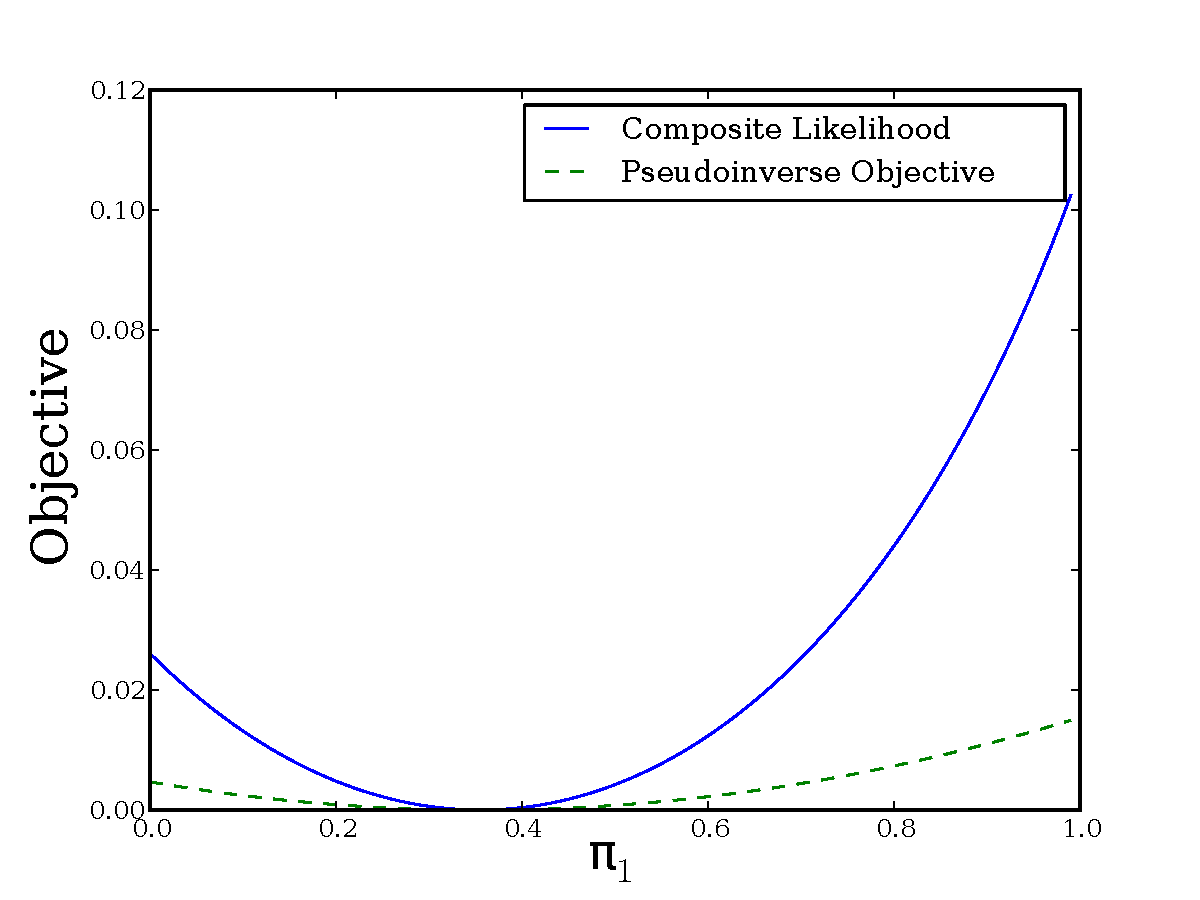
\includegraphics[width=0.45\columnwidth]{figures/piecewise-objective.pdf}
  %  }
%  \subfigure[Directed grid model] {
%    \label{fig:examples-grid}
%    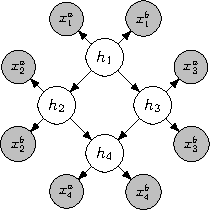
\includegraphics{figures/grid.pdf}
%  }
%  \subfigure[] {
%  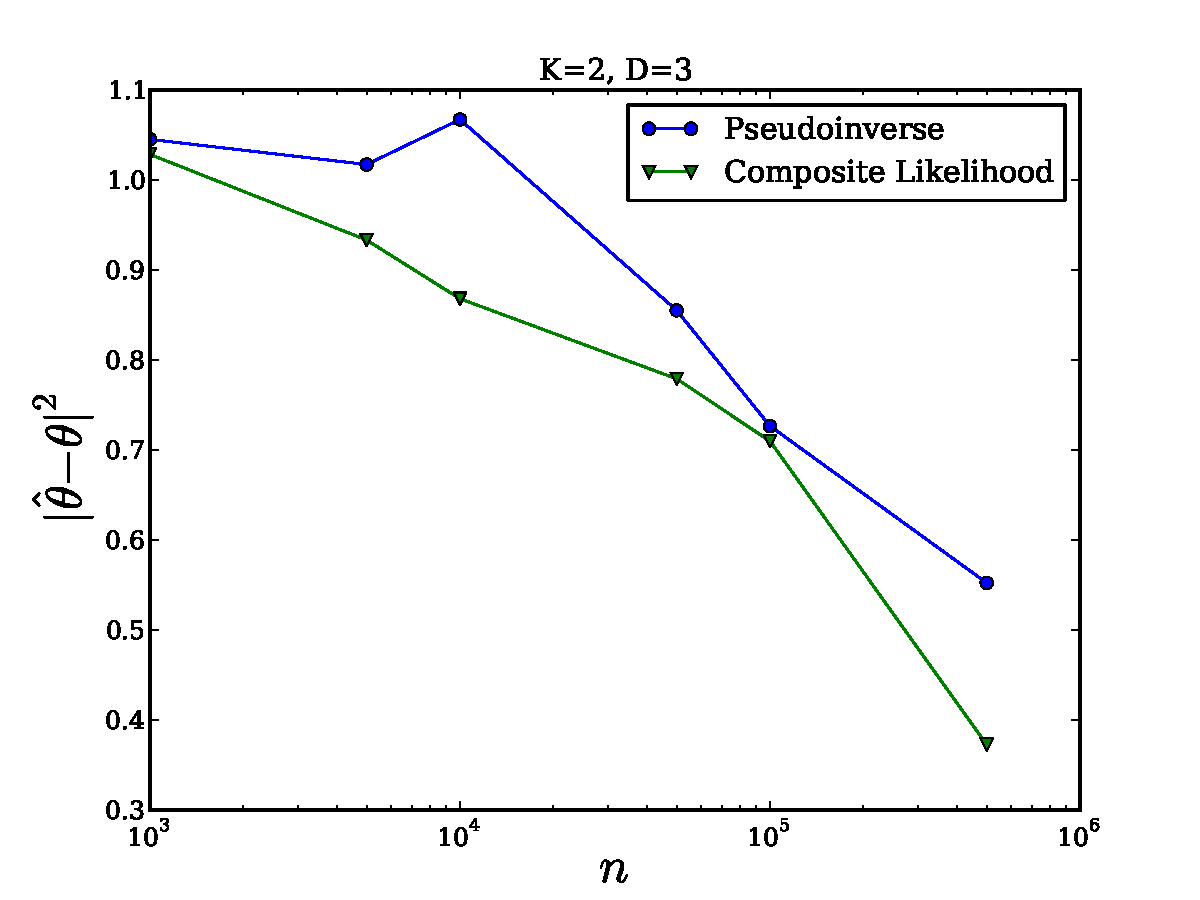
\includegraphics[width=0.8\columnwidth]{figures/hmm-2-3.pdf}
  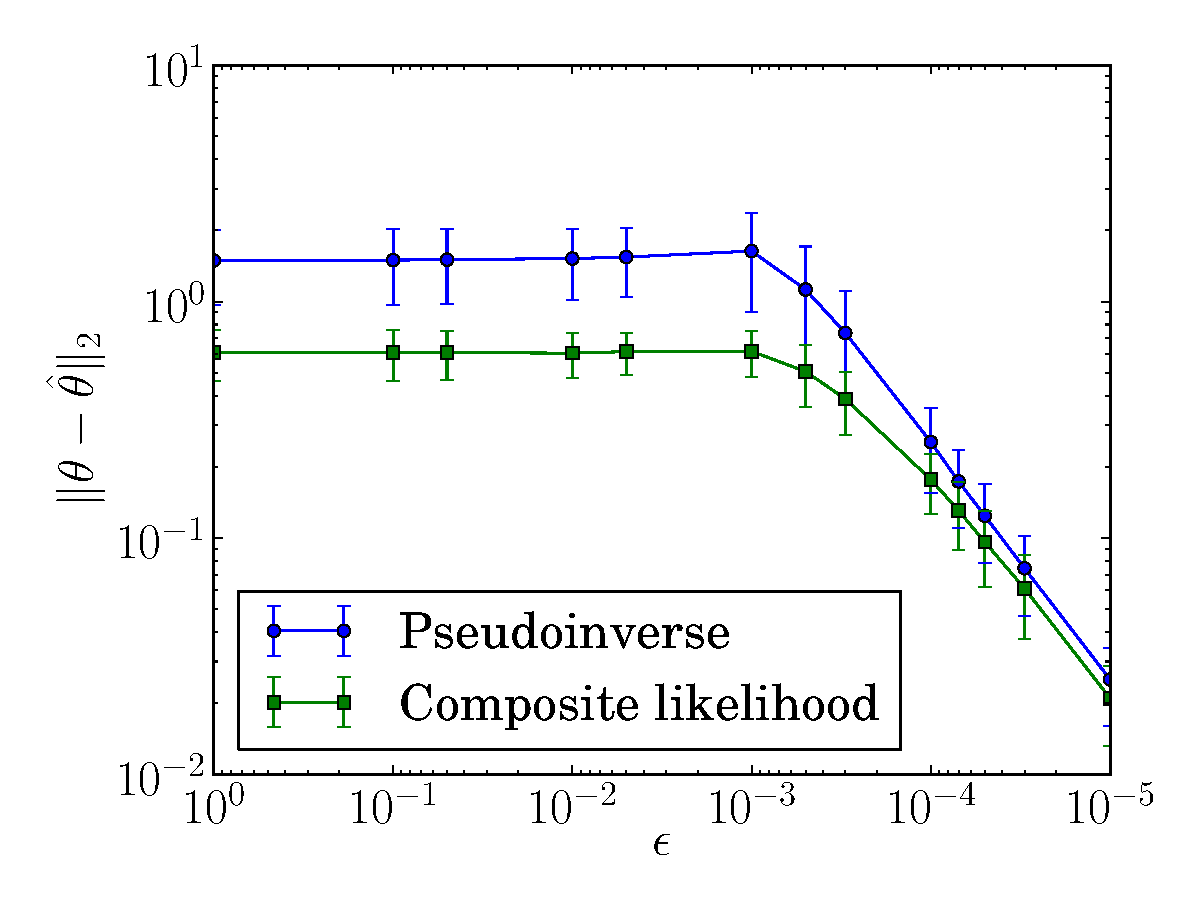
\includegraphics[width=0.8\columnwidth]{figures/asymp-k2d5.pdf}
%  }
  \caption{Parameter estimation error versus noise in moments when recovering parameters for a Hidden
  Markov Model with $k=2$ states and $d=5$ emissions using two types of estimators. Results are averaged over a 400 trials.}
    \label{fig:cl-hmm}
\end{figure}
